% vim:ft=tex

\section{Django Web Application}\label{sec:django}

% Since we only have a limited amount of time working on the project we decided to do expert based learning on Django. This means only one of us will research for the usage and implementation of Django to subsequently teach his findings to the team.
% Therefore Guillaume Goni wrote a recapitulative document for the rest of the team, so everyone could quickly get ready to work on the server code.
% It is mostly inspired by the official tutorial of Django \citep{Djangodocumentation2019} and from the Django documentation \citep{Django2019}.\\
% Due to the lack of time it wasn't`t already possible to implement the WebApp using the Django framework. This will be part of the next sprint.
% As already mentioned in chapter~\ref{sec:django} we already researched for the Django framework in the past semester, however the implementation of the Django web application was rescheduled to this part of the masterproject.

The aim of this task was to develop a web application to provide distance calculation based on our Nominatim as well as our Graphhopper server. The calculation should be done by postalcodes as well as iso codes. As a result it should return the air distance as well as the distance by route of the related postalcodes.

\subsection{Mockup}

After the requirements were clear, we designed a mockup (see figure~\ref{fig:mockup}) in order to define the layout of the web application.

\begin{figure}[H]
\centering
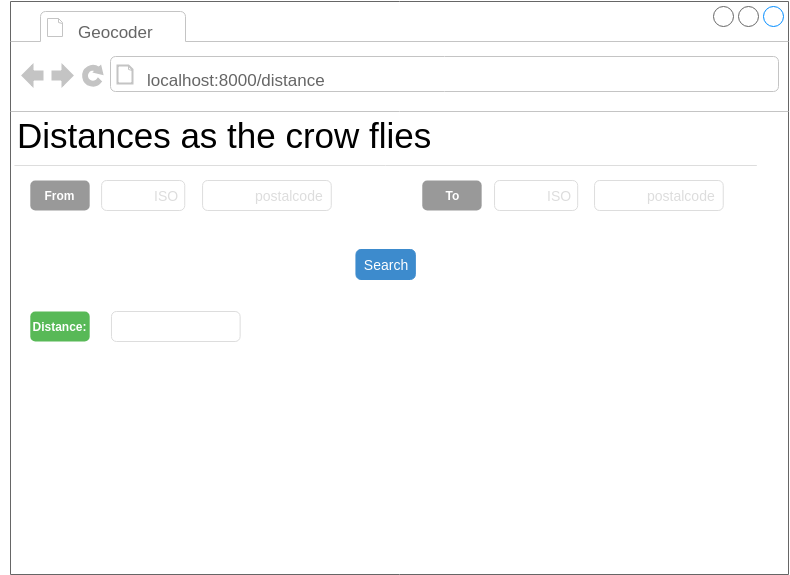
\includegraphics[width=0.8\textwidth]{img/mockup}
\captionof{figure}{Mockup for Django web app}\label{fig:mockup}
\end{figure}

The mockups shows four input fields where the user can enter the postalcode and the corresponding iso code of his start and his starting point as well as his destination. The \glqq Search\grqq-button triggers the calculation and represents the result in the input field with the label \glqq Distance\grqq below. In this mockup only the distance calculation as the crow flies was taken into consideration. However in the final web application we included the distance calculation by route as well.\\

\subsection{Implementation}

For our frontend web application, we will use \textbf{Django} as it works in python and is the most used.

\subsubsection{View}

This mockup was then implemented as an HTML file. In order to get a quick result with a sophisticated and responsive design we decided to include the Bootstrap toolkit. This open source framework provides themes, templates and code snippets for a uniform layout and rapid processing. Therefore we installed bootstrap on our Nominatim server.
The view consist mainly of four parts:
\begin{enumerate}
\item index.html
\item style.css
\item urls.py
\item views.py
\item forms.py
\end{enumerate}
The \emph{index.html} file is responsible for the general structure of the web application. The \emph{style.css} file is mainly responsible for the layout of the footer which is customized and not just adapted by bootstrap. \\
In the \emph{urls.py} we defined which HTML file should be displayed for which url. Since the web application consist of one page only we set the index.html as the entry point by calling the web application. \\
Django provides a very secure form handling which is normally a very complex business including editing the form with a convenient interface, send it to the server, validate and clean the input and then save or pass it to further processing. With Django's form functionality all this work is automated and also do it more securely then we would probably be able to do.
Therefore we created the file \emph{forms.py} where we directly specified the input fields with their corresponding length as well as if they are required or not.
\begin{lstlisting}[language=python,breaklines=true]
class CrowForm(forms.Form):
    from_zip = forms.CharField(max_length=5,required=True)
    from_iso = forms.CharField(max_length=2,required=True)
    to_zip = forms.CharField(max_length=5,required=True)
    to_iso = forms.CharField(max_length=2,required=True)
    \end{lstlisting}
The input of this form is then processed within the \emph{views.py} file, since here the post and get requests are handled.
The \emph{views.py} file is responsible to handle post ad get requests.
This file calls also the responsible methods of the datamodel in order to calculate the distances.
Moreover it returns the results to the input fields \glqq Direct\grqq and \glqq By route\grqq which can be seen in figure~\ref{fig:webapp}.
\begin{figure}[H]
\hspace{-2.0cm}
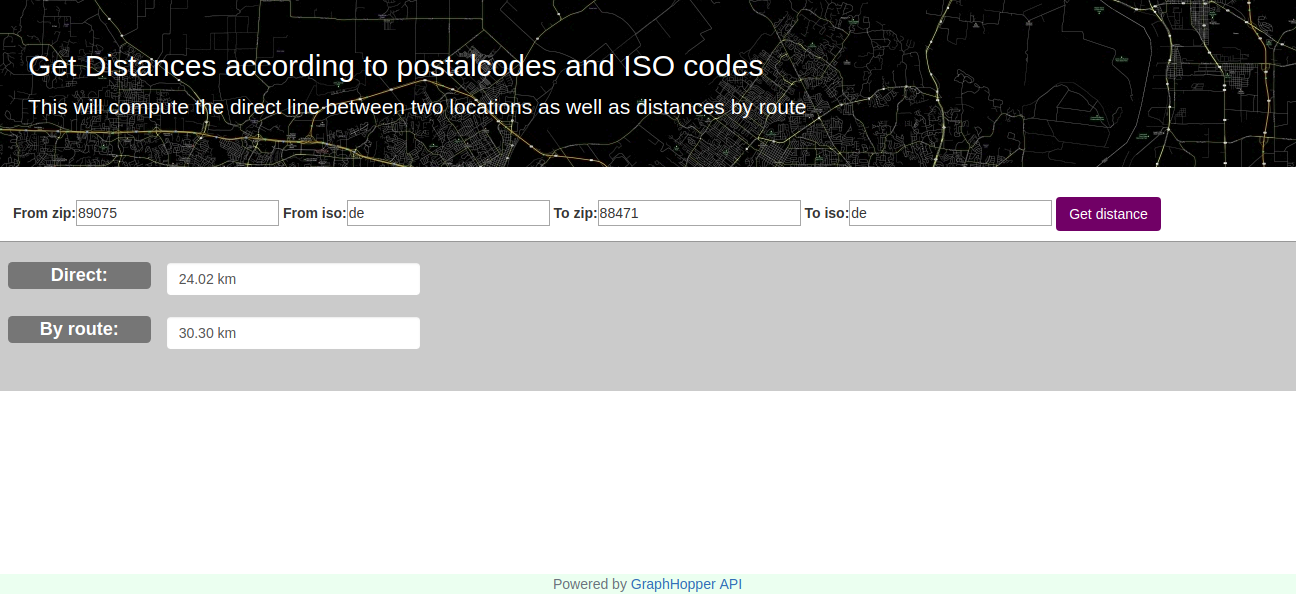
\includegraphics[width=1.3\textwidth]{img/webapp}
\captionof{figure}{Final layout of the Django web application}\label{fig:webapp}
\end{figure}

%%%%%%%%%%%%%%%%%%%%%%%%%%%%%%%%%%%%%%%%%%%%%%%%%%%%%%%%%%%%%%%%%%%%%%%%%%%%%%%%%%%%%%%%%%%%%%
%%%%%%%%%Have fun Guillaume no it is your turn:-)%%%%%%%%%%%%%%%%%%%%%%%%%%%%%%%%%%%%%%%%%%%%%
\subsubsection{Calculation}

%%%%%%%%%%%%%%%%%%%%%%%%%%%%%%%%%%%%%%%%%%%%%%%%%%%%%%%%%%%%%%%%%%%%%%%%%%%%%%%%%%%%%%%%%%%%%%
%please add here the calculation bla bla bla
